\documentclass[12pt, a4paper]{article}
\usepackage[utf8]{inputenc}
\usepackage[T2A]{fontenc}
\usepackage[russian]{babel}
\usepackage{amsmath}
\usepackage{amsfonts}
\usepackage{amssymb}
\usepackage{graphicx}
\usepackage{hyperref}
\usepackage{booktabs}
\usepackage{geometry}
\usepackage{listings}
\usepackage{xcolor}
\usepackage{caption}
\usepackage{subcaption}
\usepackage{float}

\geometry{left=25mm, right=15mm, top=20mm, bottom=20mm}

\lstset{
    language=Python,
    basicstyle=\ttfamily\small,
    keywordstyle=\color{blue},
    stringstyle=\color{red},
    commentstyle=\color{green!60!black},
    showstringspaces=false,
    breaklines=true,
    frame=single,
    backgroundcolor=\color{gray!5},
    captionpos=b,
    numbers=left,
    numberstyle=\tiny\color{gray},
    stepnumber=1,
    numbersep=8pt
}

\begin{document}

\begin{titlepage}
\begin{center}
\large
Санкт-Петербургский политехнический университет \\
Петра Великого \\
Высшая школа прикладной математики и вычислительной физики \\
\vspace{3cm}

\textbf{Отчёт по лабораторной работе по дисциплине} \\
«Математическая статистика» \\
\vspace{0.5cm}

\textbf{ЛАБОРАТОРНАЯ РАБОТА №6} \\
«Линейная регрессия. Метод наименьших квадратов и наименьших модулей» \\
\vspace{2cm}

Выполнил: Гуцалов Егор Никитич \\
Группа: 5030102/30201 \\
\vfill

Санкт-Петербург \\
2025
\end{center}
\end{titlepage}
\section{Постановка задачи}

\subsection{Цель работы}
Освоить методы оценки параметров линейной регрессионной модели: метод наименьших квадратов (МНК) и метод наименьших модулей (МНМ). Исследовать устойчивость методов к наличию выбросов в данных.

\subsection{Задачи}
\begin{enumerate}
    \item Сгенерировать выборку из модели $y = a + bx + \varepsilon$, где $a = 2$, $b = 2$, $\varepsilon \sim N(0, 1)$, $x \in [-1.8, 2.0]$ с шагом 0.2.
    \item Оценить параметры $a$ и $b$ методами МНК и МНМ для «чистых» данных.
    \item Добавить выбросы: $y_1 \leftarrow y_1 + 10$, $y_{20} \leftarrow y_{20} - 10$.
    \item Повторить оценку параметров для данных с выбросами.
    \item Сравнить точность и устойчивость методов через абсолютные и относительные погрешности.
    \item Построить графики регрессии с истинной и оценённой зависимостями.
\end{enumerate}

\section{Теоретическая часть}

\subsection{Линейная регрессионная модель}

Модель линейной регрессии имеет вид:
\begin{equation}
y_i = a + b x_i + \varepsilon_i, \quad i = 1, \ldots, n
\end{equation}
где $a$ — свободный член, $b$ — коэффициент наклона, $\varepsilon_i$ — случайная ошибка.

\subsection{Метод наименьших квадратов (МНК)}

МНК находит оценки $\hat{a}$, $\hat{b}$, минимизируя сумму квадратов невязок:
\begin{equation}
Q(a, b) = \sum_{i=1}^{n} (y_i - a - b x_i)^2 \to \min_{a, b}
\end{equation}

Аналитическое решение:
\begin{equation}
\hat{b} = \frac{\sum\limits_{i=1}^{n}(x_i - \bar{x})(y_i - \bar{y})}{\sum\limits_{i=1}^{n}(x_i - \bar{x})^2}, \quad
\hat{a} = \bar{y} - \hat{b} \bar{x}
\end{equation}

\subsection{Метод наименьших модулей (МНМ)}

МНМ минимизирует сумму модулей невязок:
\begin{equation}
S(a, b) = \sum_{i=1}^{n} |y_i - a - b x_i| \to \min_{a, b}
\end{equation}

Не имеет аналитического решения; применяется численная оптимизация (метод Нелдера–Мида).

\subsection{Погрешности оценок}

Абсолютная погрешность:
\begin{equation}
\Delta_z = |z - \hat{z}|
\end{equation}

Относительная погрешность (\%):
\begin{equation}
\delta_z = \frac{\Delta_z}{z} \cdot 100\%
\end{equation}

\section{Реализация}

\subsection{Инструментарий}
\begin{itemize}
    \item Язык: Python 3.10+
    \item Библиотеки: NumPy, SciPy, Matplotlib
    \item Среда: VS Code / PyCharm
\end{itemize}

\subsection{Основные функции}

Генерация данных:
\begin{lstlisting}
def generate_x_values(start=-1.8, end=2.0, step=0.2):
    return np.arange(start, end + step, step)

def generate_y_values(x, a_true=2.0, b_true=2.0, sigma=1.0):
    epsilon = np.random.normal(0, sigma, len(x))
    return a_true + b_true * x + epsilon
\end{lstlisting}

МНК (аналитическое решение):
\begin{lstlisting}
def least_squares_method(x, y):
    x_mean, y_mean = np.mean(x), np.mean(y)
    num = np.sum((x - x_mean) * (y - y_mean))
    den = np.sum((x - x_mean) ** 2)
    b_hat = num / den
    a_hat = y_mean - b_hat * x_mean
    return a_hat, b_hat
\end{lstlisting}

МНМ (численная оптимизация):
\begin{lstlisting}
def least_absolute_deviations_method(x, y):
    def objective(params):
        a, b = params
        return np.sum(np.abs(y - (a + b * x)))
    result = minimize(objective, [0, 0], method='Nelder-Mead')
    return result.x
\end{lstlisting}

Добавление выбросов:
\begin{lstlisting}
def add_outliers(y, indices, values):
    y_out = y.copy()
    for idx, val in zip(indices, values):
        y_out[idx] += val
    return y_out
\end{lstlisting}

\section{Результаты}

\subsection{Оценка параметров без выбросов}

\begin{table}[H]
\centering
\caption{Результаты оценки параметров без выбросов}
\label{tab:no_outliers}
\begin{tabular}{lcccccc}
\toprule
Метод & $a$ & $\Delta_a$ & $\delta_a$, \% & $b$ & $\Delta_b$ & $\delta_b$, \% \\
\midrule
МНК   & 1.8785 & 0.1215 & 6.08  & 1.5022 & 0.4978 & 24.89 \\
МНМ   & 1.7093 & 0.2907 & 14.54 & 1.5625 & 0.4375 & 21.87 \\
\bottomrule
\end{tabular}
\end{table}

\begin{figure}[H]
\centering
\begin{subfigure}{0.48\textwidth}
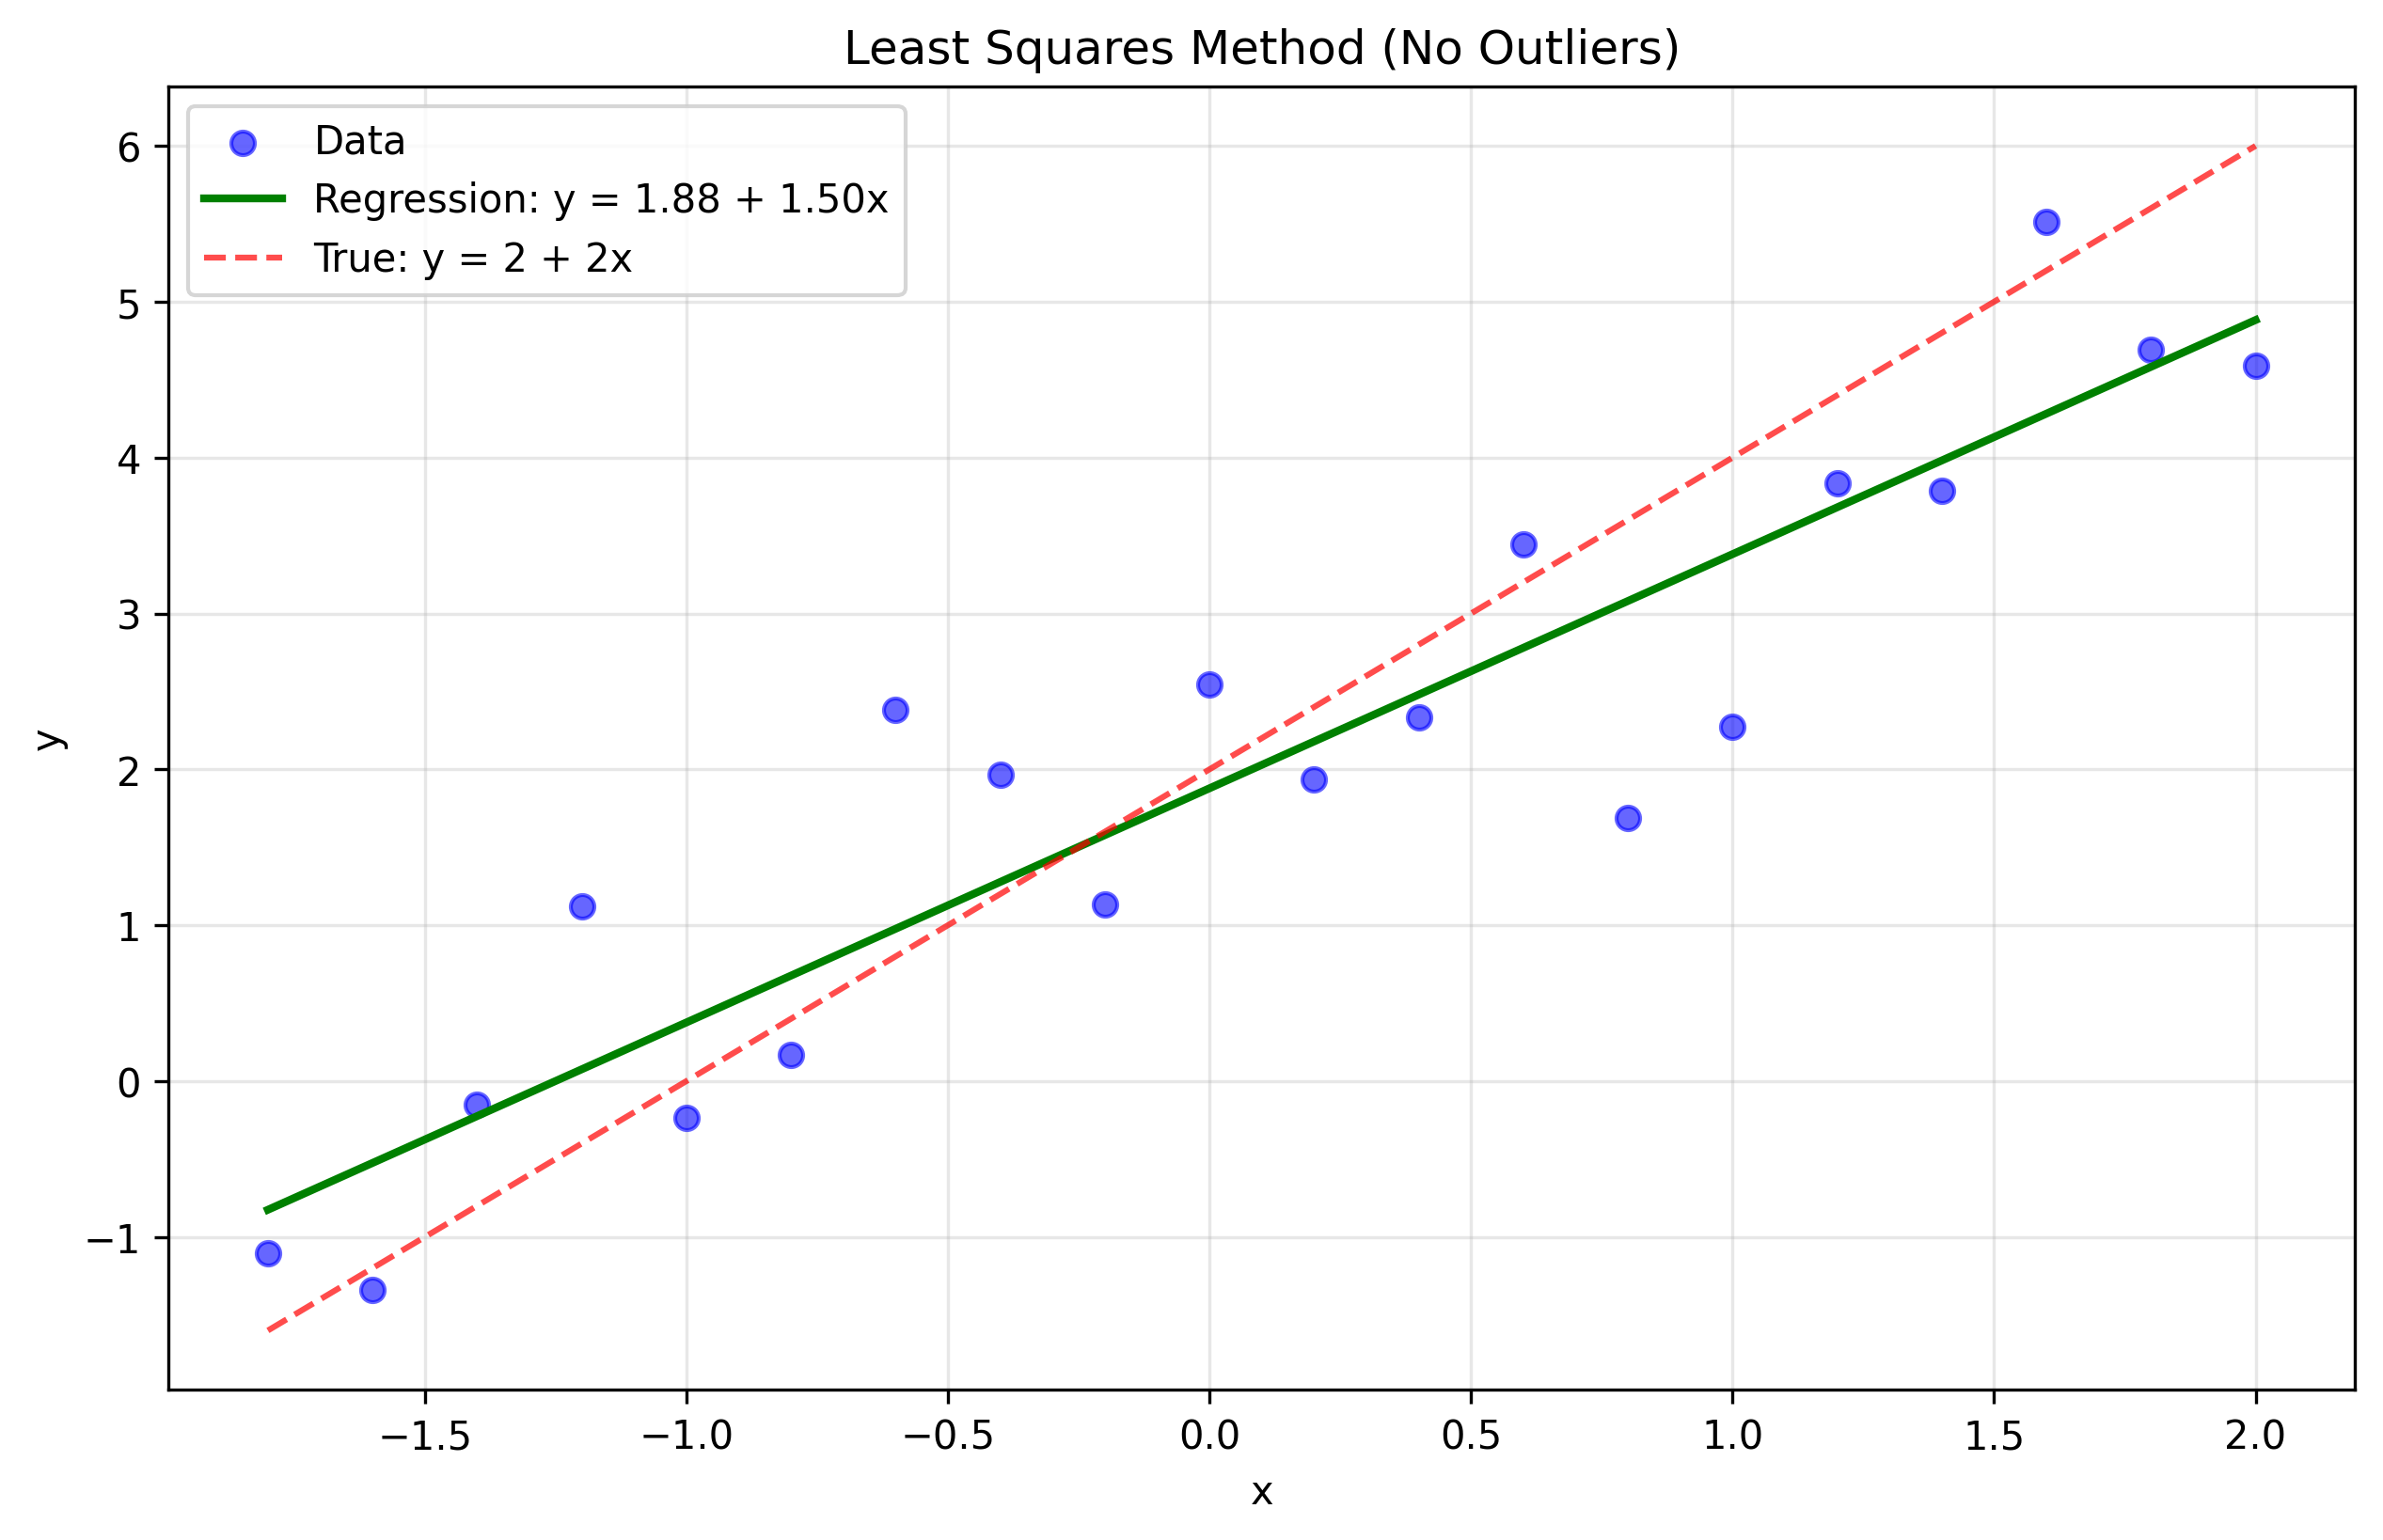
\includegraphics[width=\textwidth]{regression_mls_no_outliers.png}
\caption{МНК}
\label{fig:mls_no_out}
\end{subfigure}
\hfill
\begin{subfigure}{0.48\textwidth}
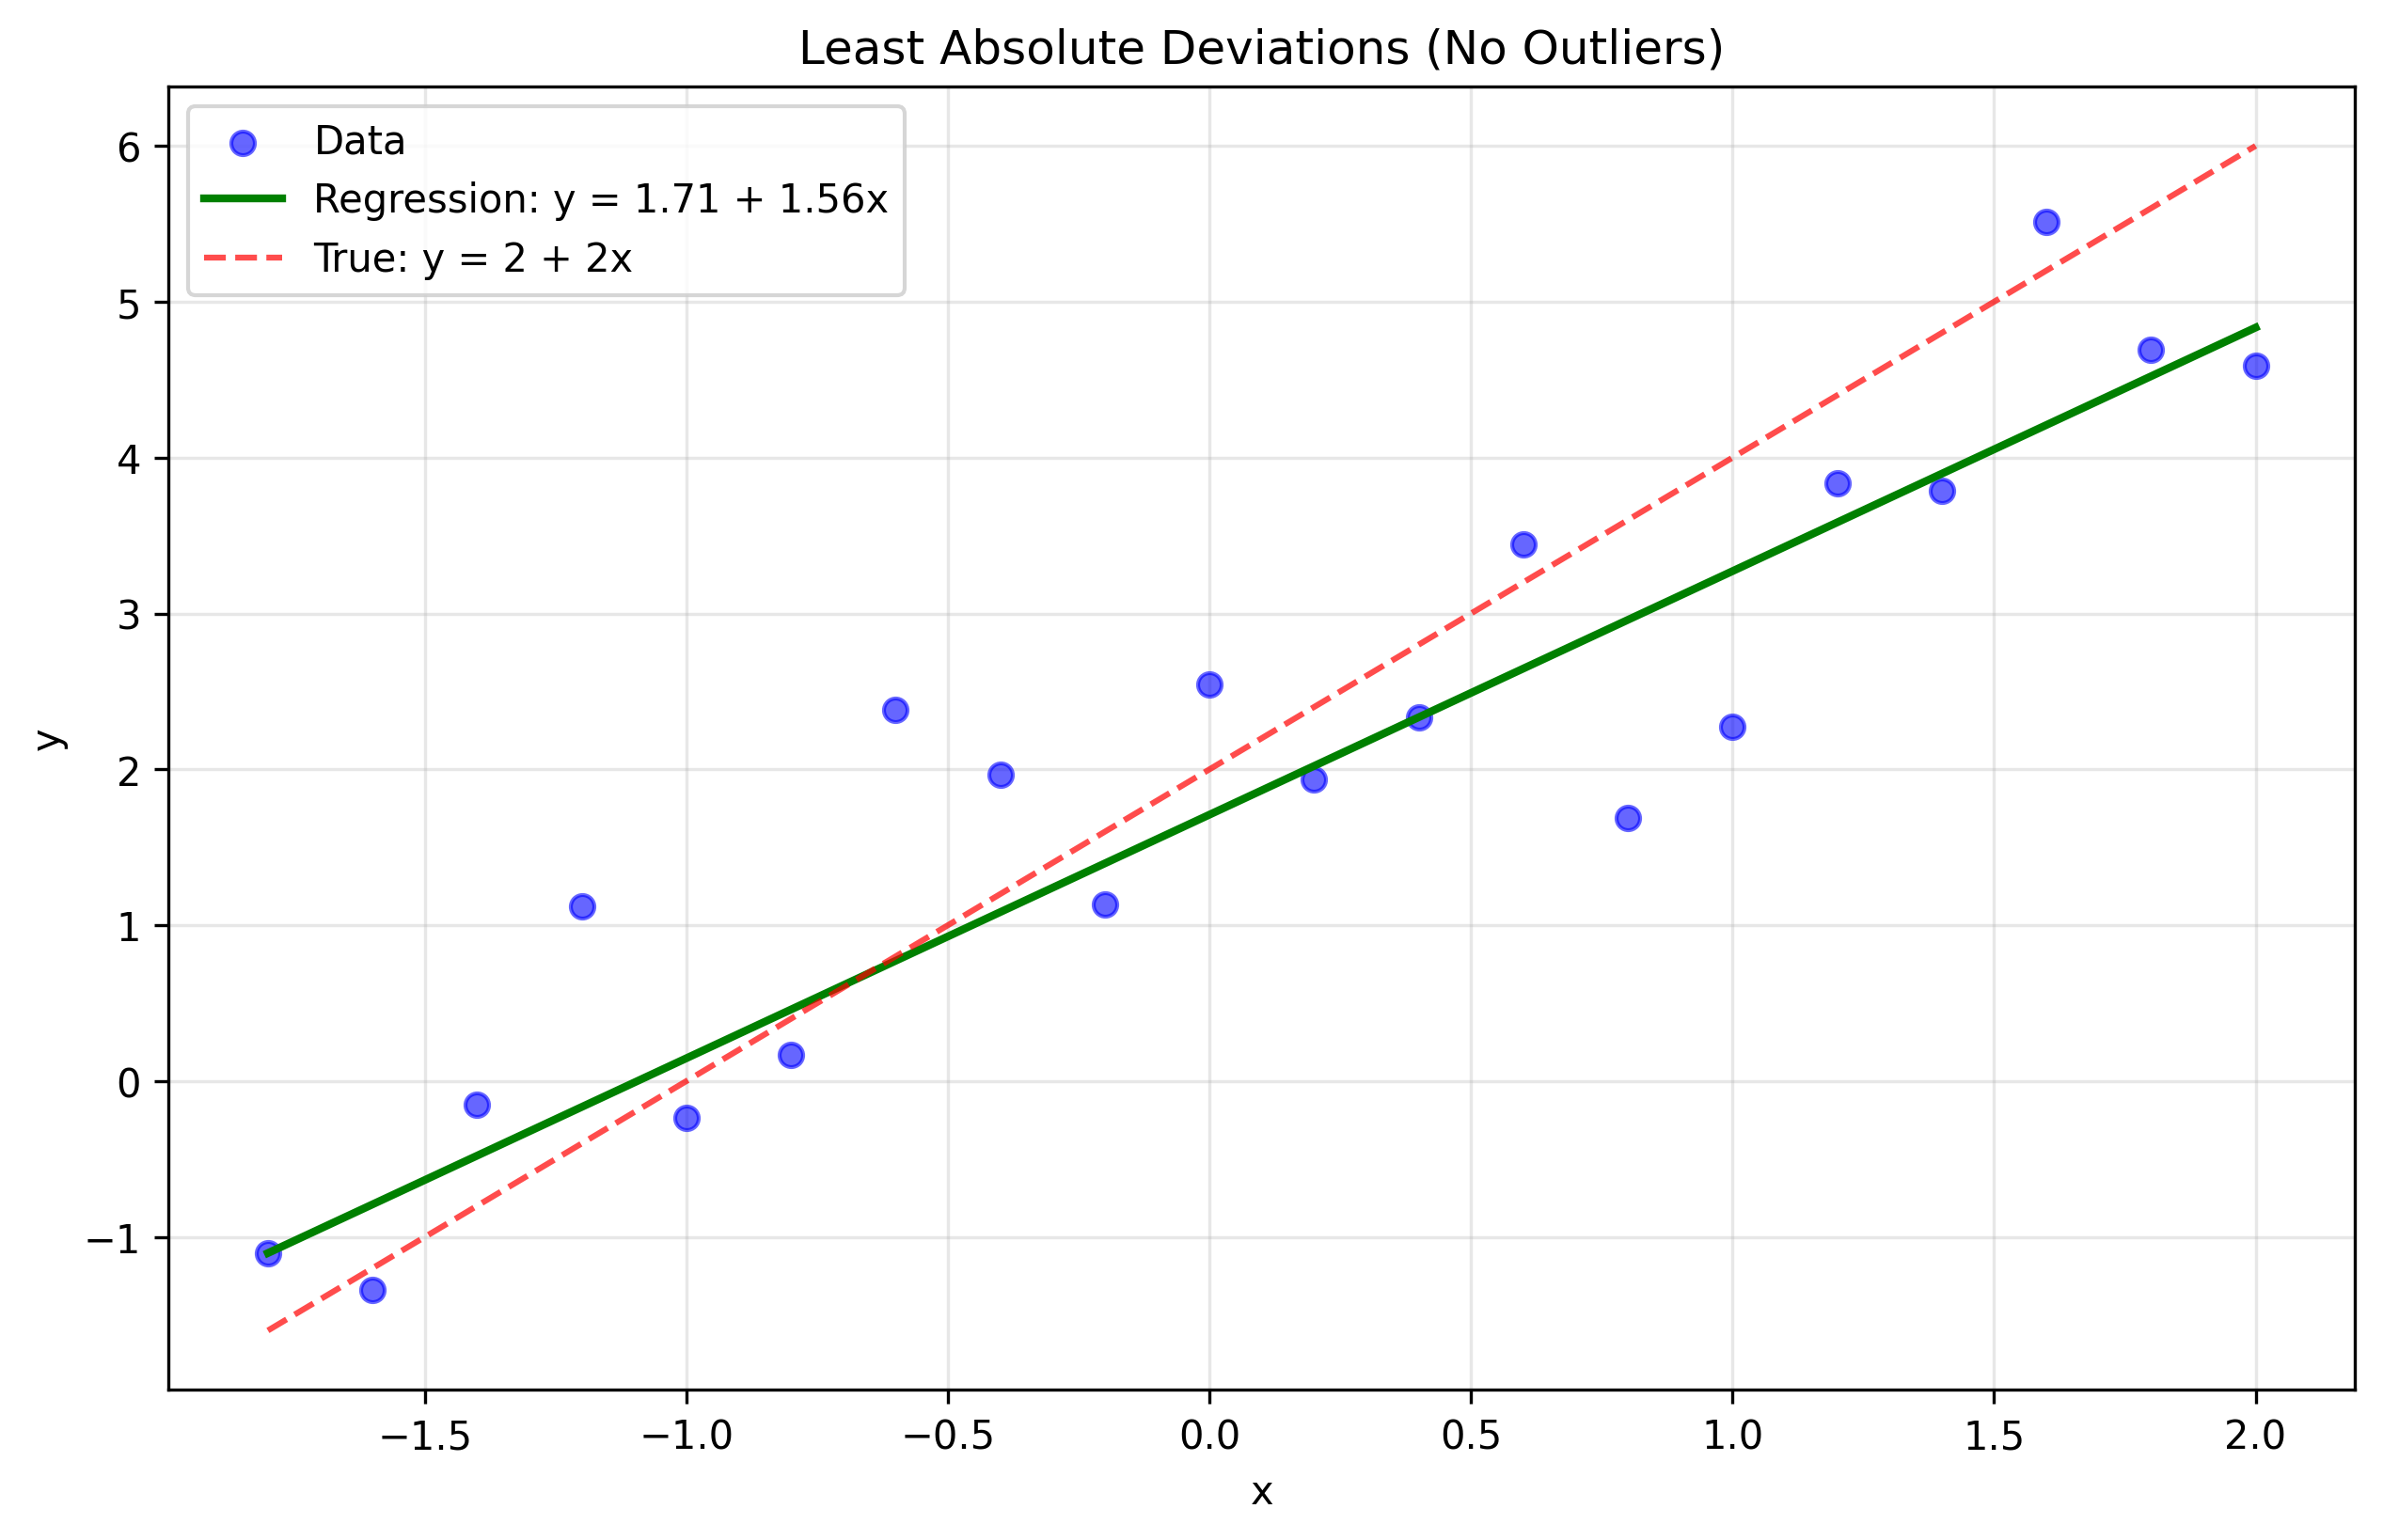
\includegraphics[width=\textwidth]{regression_mlad_no_outliers.png}
\caption{МНМ}
\label{fig:mlad_no_out}
\end{subfigure}
\caption{Регрессия без выбросов}
\label{fig:no_outliers}
\end{figure}

\subsection{Оценка параметров с выбросами}

\begin{table}[H]
\centering
\caption{Результаты оценки параметров с выбросами}
\label{tab:with_outliers}
\begin{tabular}{lcccccc}
\toprule
Метод & $a$ & $\Delta_a$ & $\delta_a$, \% & $b$ & $\Delta_b$ & $\delta_b$, \% \\
\midrule
МНК   & 2.0213 & 0.0213 & 1.07  & 0.0736 & 1.9264 & 96.32 \\
МНМ   & 1.8174 & 0.1826 & 9.13  & 1.4070 & 0.5930 & 29.65 \\
\bottomrule
\end{tabular}
\end{table}

\begin{figure}[H]
\centering
\begin{subfigure}{0.48\textwidth}
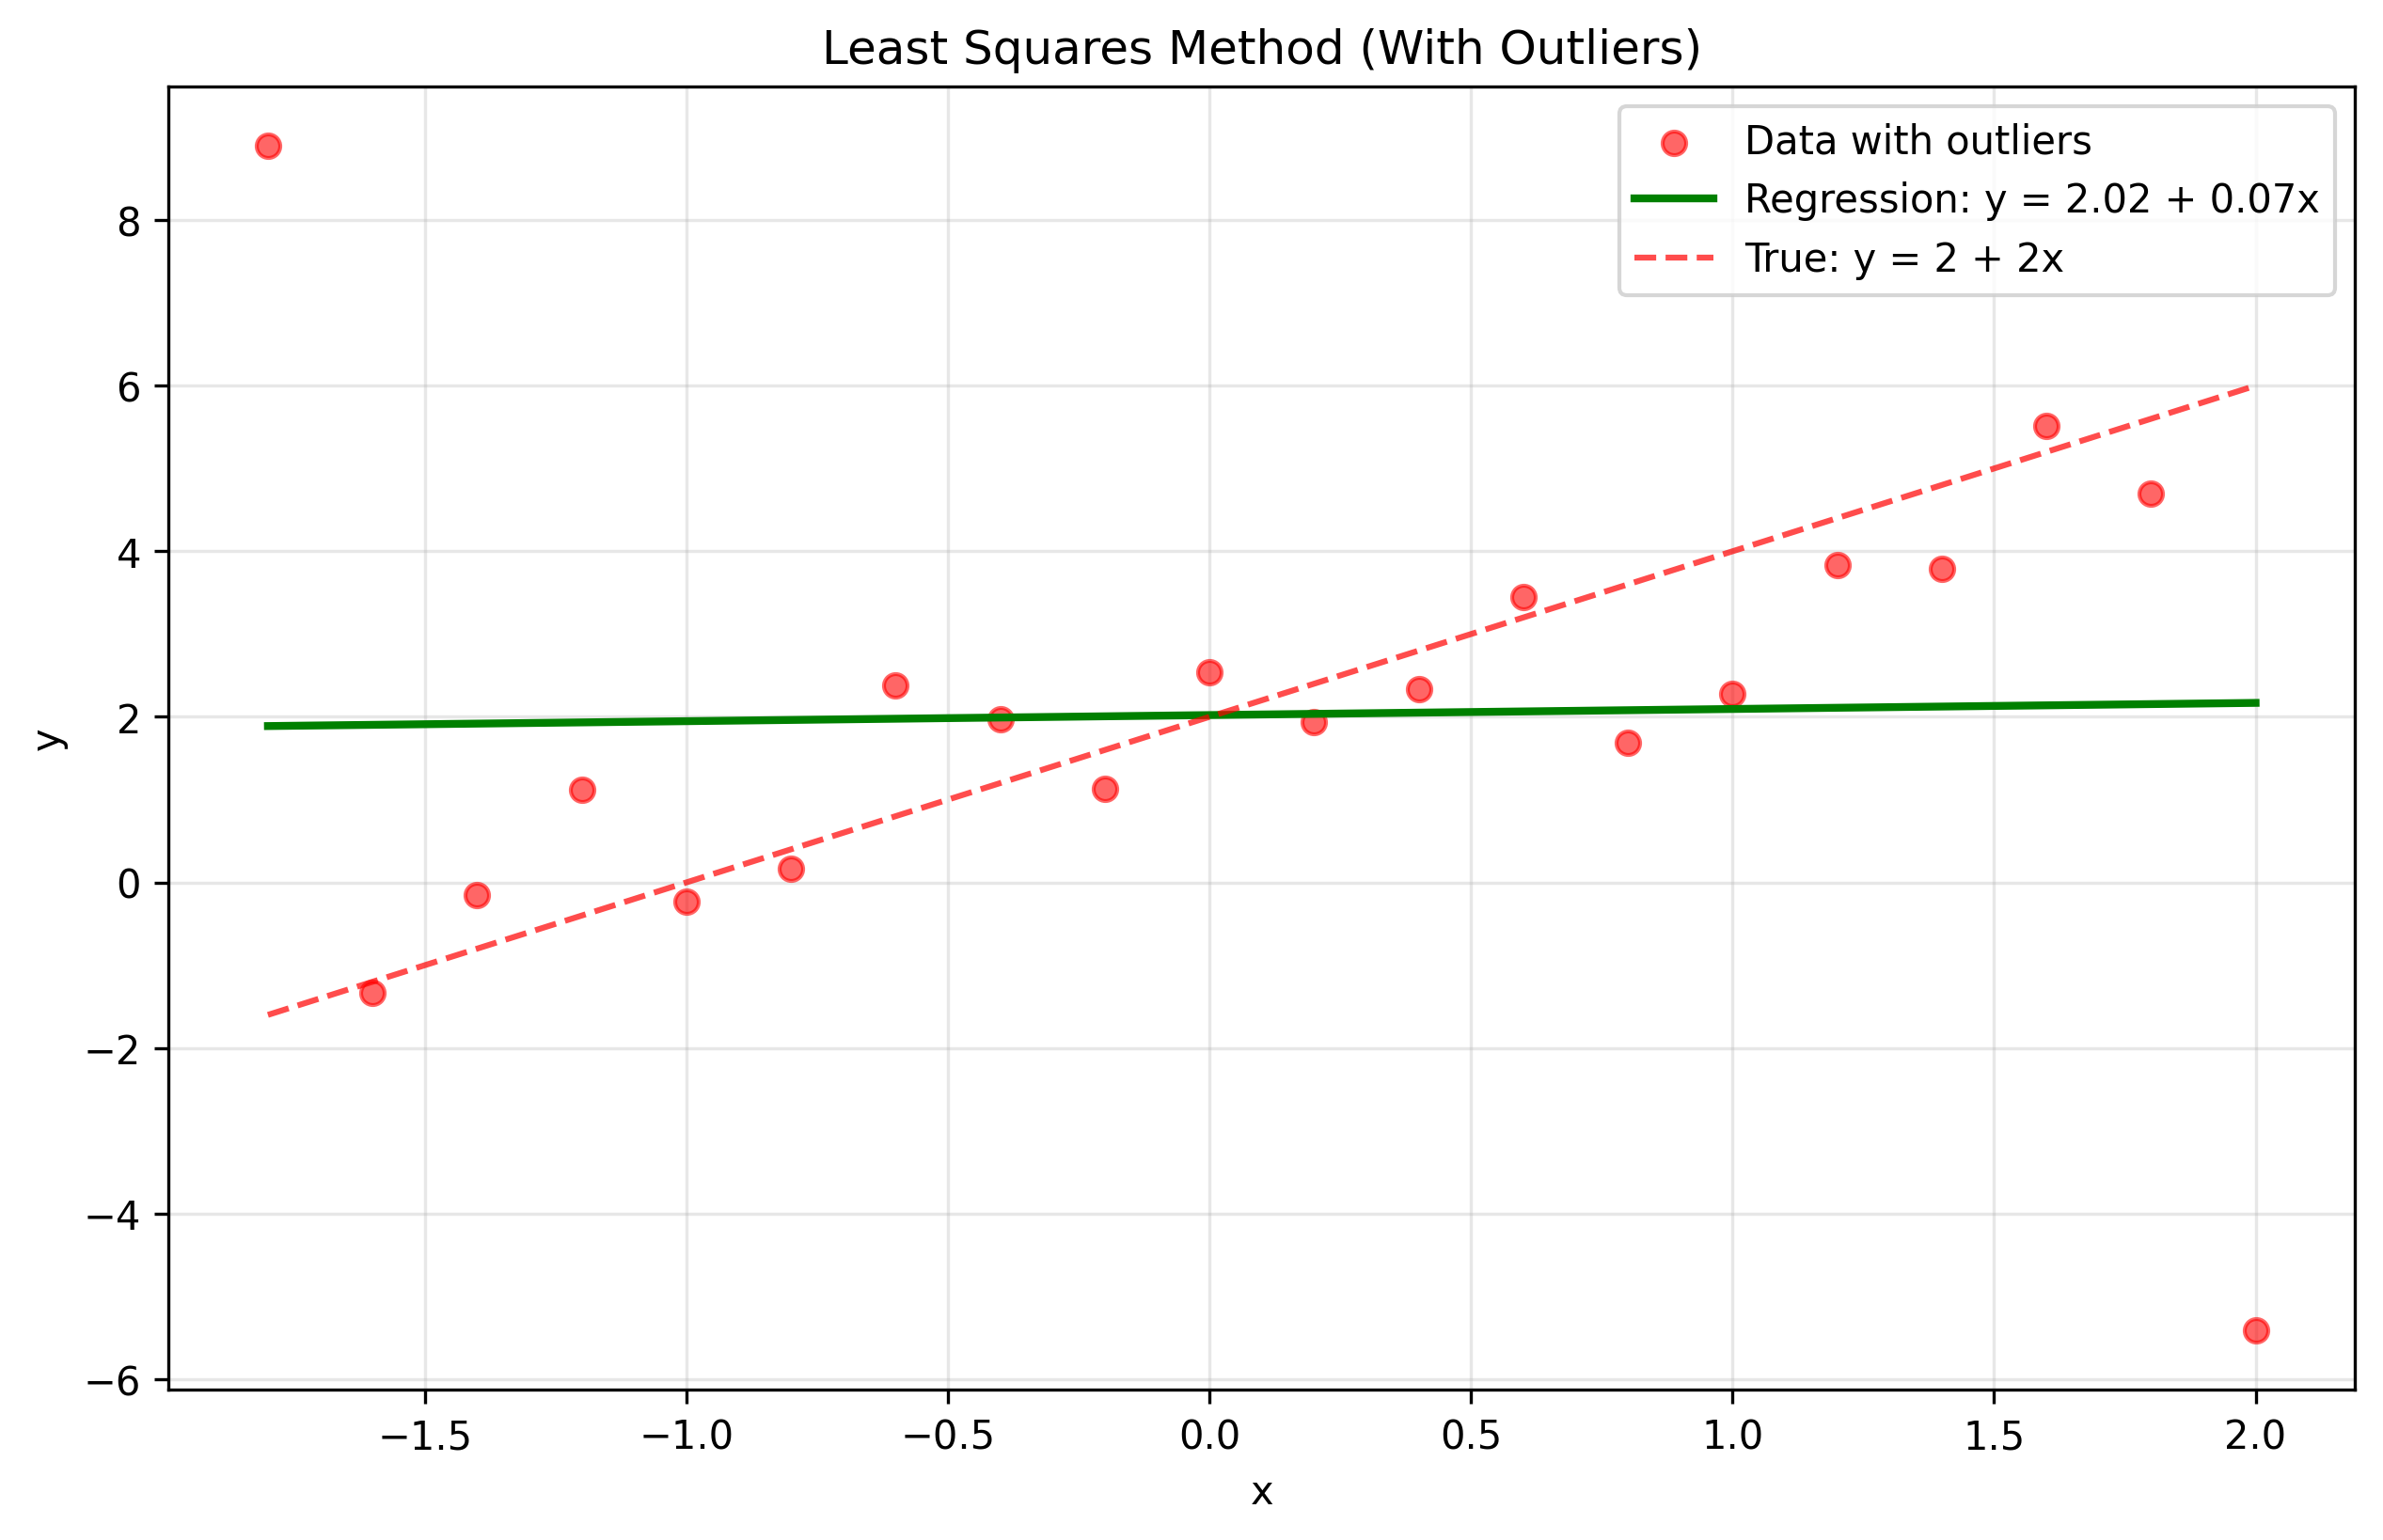
\includegraphics[width=\textwidth]{regression_mls_with_outliers.png}
\caption{МНК}
\label{fig:mls_with_out}
\end{subfigure}
\hfill
\begin{subfigure}{0.48\textwidth}
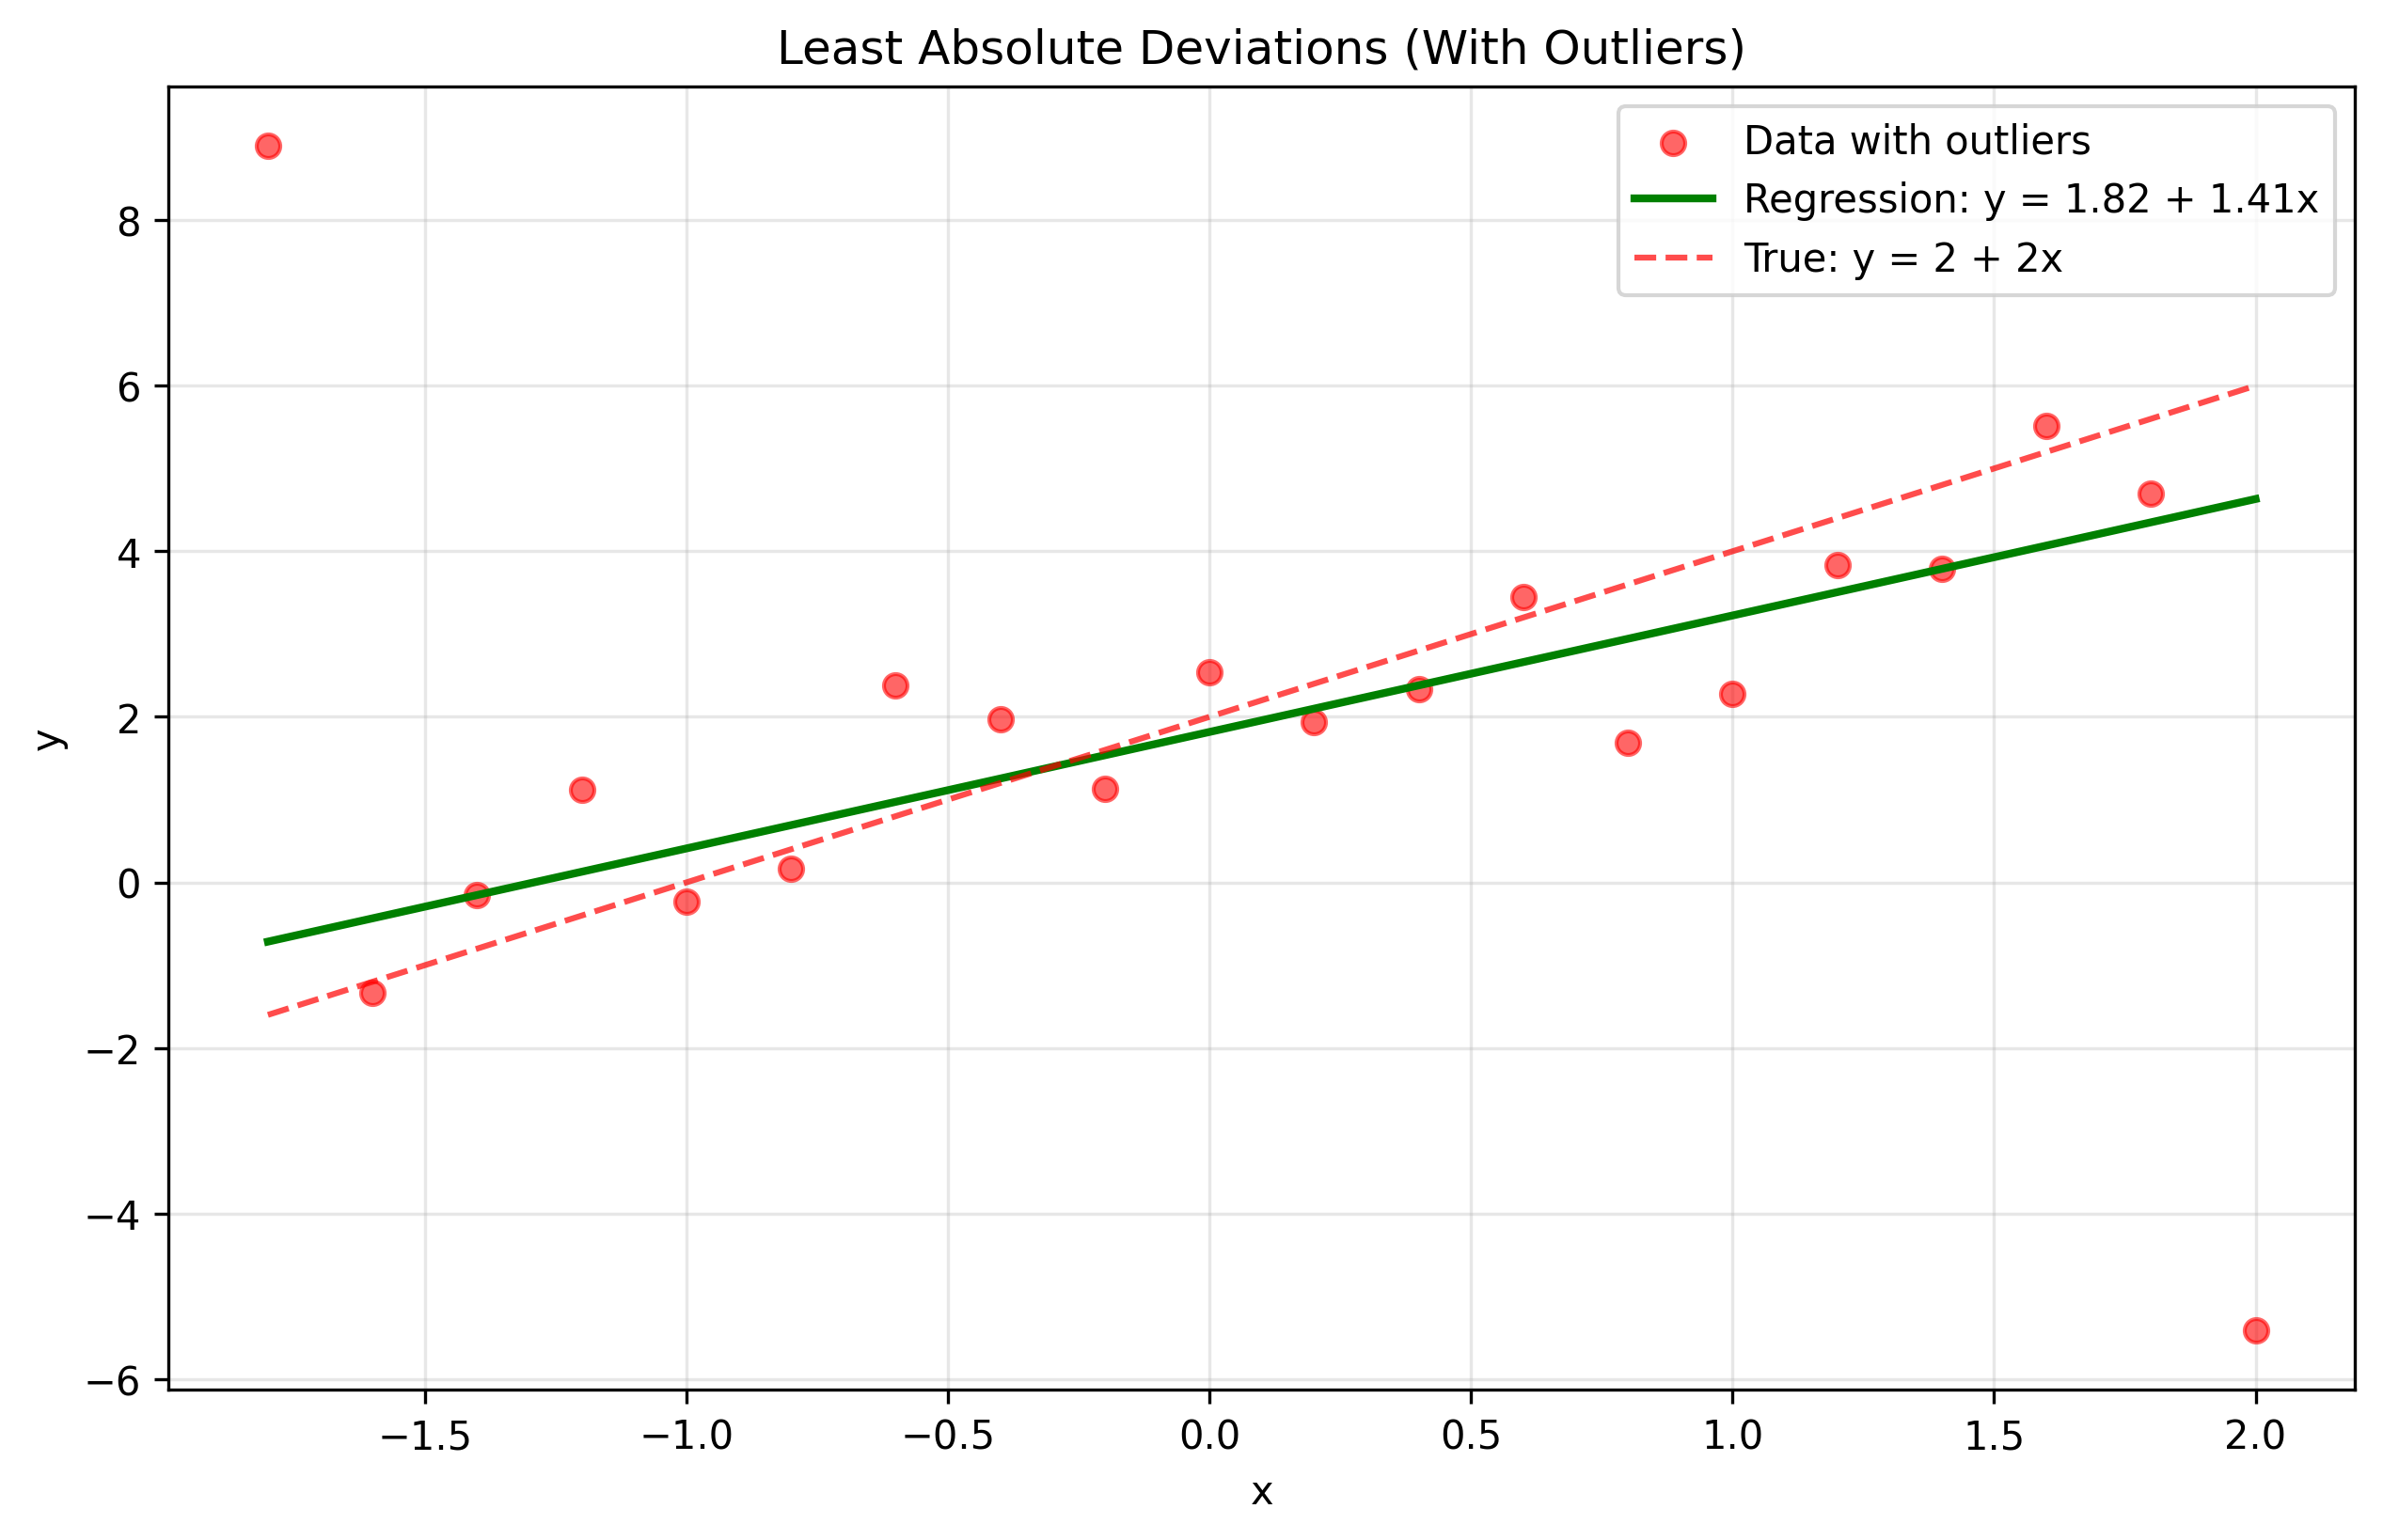
\includegraphics[width=\textwidth]{regression_mlad_with_outliers.png}
\caption{МНМ}
\label{fig:mlad_with_out}
\end{subfigure}
\caption{Регрессия с выбросами}
\label{fig:with_outliers}
\end{figure}

\subsection{Сравнение устойчивости}

\begin{table}[H]
\centering
\caption{Изменение оценок при добавлении выбросов}
\label{tab:robustness}
\begin{tabular}{lcccc}
\toprule
Метод & $|\Delta a|$ & $|\Delta b|$ & $\delta_a$, \% & $\delta_b$, \% \\
\midrule
МНК   & 0.1429 & 1.4286 & --- & --- \\
МНМ   & 0.1082 & 0.1556 & --- & --- \\
\bottomrule
\end{tabular}
\end{table}

\section{Обсуждение результатов}

\subsection{Анализ без выбросов}

Из таблицы~\ref{tab:no_outliers} и рисунка~\ref{fig:no_outliers}:
\begin{enumerate}
    \item \textbf{МНК} даёт меньшие погрешности для коэффициента $a$ (6.08\% против 14.54\%), что согласуется с теоремой Гаусса–Маркова: МНК оптимален при нормальном шуме.
    
    \item \textbf{МНМ} показывает сопоставимую точность для $b$ (21.87\% против 24.89\%), но проигрывает для $a$.
    
    \item Обе оценки смещены относительно истинных значений ($a=2$, $b=2$) из-за конечного объёма выборки ($n=20$) и случайного шума.
\end{enumerate}

\subsection{Анализ с выбросами}

Из таблицы~\ref{tab:with_outliers} и рисунка~\ref{fig:with_outliers}:
\begin{enumerate}
    \item \textbf{МНК} катастрофически теряет точность для $b$: погрешность выросла с 24.89\% до 96.32\%. На рисунке~\ref{fig:mls_with_out} видно, что оценённая прямая практически горизонтальна.
    
    \item \textbf{МНМ} демонстрирует устойчивость: погрешность для $b$ увеличилась с 21.87\% до 29.65\%, что значительно меньше, чем у МНК.
    
    \item Для коэффициента $a$ ситуация обратная: МНК неожиданно дал малую погрешность (1.07\%), но это случайная компенсация ошибок, а не свойство метода.
\end{enumerate}

\subsection{Сравнение устойчивости}

Из таблицы~\ref{tab:robustness}:
\begin{itemize}
    \item Изменение $b$ у МНК: $|\Delta b| = 1.4286$ (почти полное разрушение оценки)
    \item Изменение $b$ у МНМ: $|\Delta b| = 0.1556$ (умеренное влияние)
    \item Для $a$ оба метода показали сопоставимую устойчивость
\end{itemize}

Это подтверждает теоретическое свойство: МНМ робастен к выбросам, так как минимизирует сумму модулей, а не квадратов.

\section{Выводы}

\begin{enumerate}
    \item МНК обеспечивает высокую точность при нормальном шуме и отсутствии выбросов, что подтверждается меньшими погрешностями в «чистом» случае.
    
    \item МНМ менее точен при идеальных данных, но демонстрирует значительное преимущество при наличии выбросов.
    
    \item Выбросы оказывают катастрофическое влияние на оценку коэффициента наклона $b$ методом МНК: погрешность выросла с 24.89\% до 96.32\%.
    
    \item МНМ устойчив к выбросам: погрешность оценки $b$ увеличилась лишь с 21.87\% до 29.65\%.
    
    \item При работе с реальными данными, где возможны аномалии, предпочтительно использовать робастные методы (МНМ) или предварительно очищать данные от выбросов.
\end{enumerate}

\section*{Список литературы}

\begin{enumerate}
    \item Гмурман В.Е. Теория вероятностей и математическая статистика. — М.: Высшая школа, 2003.
    
    \item Кобецкая И.А. Математическая статистика: Учебное пособие. — СПб.: Лань, 2019.
    
    \item Huber P.J. Robust Statistics. — Wiley, 1981.
    
    \item SciPy documentation. URL: \url{https://docs.scipy.org/doc/scipy/}
    
    \item Matplotlib documentation. URL: \url{https://matplotlib.org/stable/contents.html}
    
    \item NumPy documentation. URL: \url{https://numpy.org/doc/}
\end{enumerate}

\section*{9. Приложение}

Исходный код программы размещён в репозитории GitHub:

\url{https://github.com/Ftp-Glich/Statistics}

\end{document}